\documentclass[11pt]{article}
\usepackage[utf8]{inputenc}
\usepackage{amssymb, amsmath, amsthm, changepage, graphicx, caption, subcaption, ulsy}
\usepackage{amssymb}
\usepackage{mathrsfs}
\usepackage{comment}
\excludecomment{ignore}
\includecomment{solution}
\includecomment{question}
\def\nats {{\mathbb N}}
\def\ints {{\mathbb Z}}
\newcommand{\Implies}{\mbox{ IMPLIES }}
\newcommand{\Or}{\mbox{ OR }}
\newcommand{\Andd}{\mbox{ AND }}
\newcommand{\Not}{\mbox{NOT }}
\newcommand{\Iff}{\mbox{ IFF }}
\newcommand{\True}{\mbox{T}}
\newcommand{\False}{\mbox{F}}
\newcommand{\Subsets}[1]{\mathscr{P}_{#1}(\{1,\ldots N\})}

\graphicspath{{./images/}}

\title{MAT157 Problem Set 13}
\author{Nicolas}

\newcommand{\R}{\mathbb{R}}

\newcommand{\N}{\mathbb{N}}

\newcommand{\Z}{\mathbb{Z}}

\newcommand{\F}{\mathbb{F}}

\newcommand{\C}{\mathbb{C}}

\newcommand{\Q}{\mathbb{Q}}

\newcommand{\nskip}{\\ \bigskip}

\newcommand{\norm}[1]{\left\lVert#1\right\rVert}

\newcommand{\inn}[2]{\langle#1,#2\rangle}


\newenvironment{myproof}
{\begin{proof} \begin{adjustwidth}{3em}{0pt}$ $\par\nobreak\ignorespaces}
{\end{adjustwidth} \end{proof}} 

\begin{document}

\maketitle
\begin{flushleft}

1.

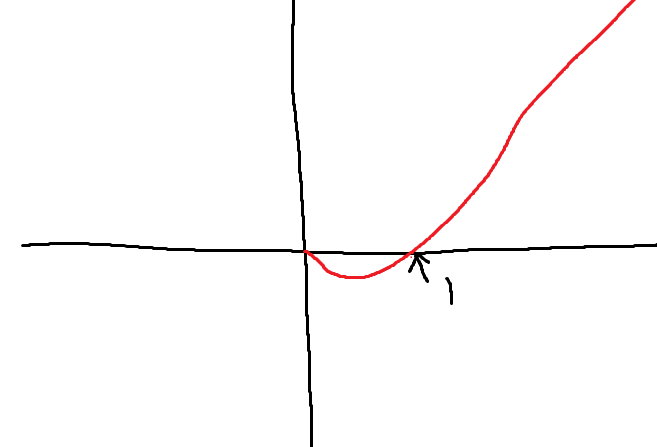
\includegraphics[width=\textwidth]{shittyxlogx.png}

\begin{align*}
f(x) = & \ x \log x \\
f'(x) = & \ 1 + \log x \\
f''(x) = & \ \frac{1}{x}
\end{align*}
$f$ is increasing on $(\frac1e, \infty)$ because $f'$ is positive on that ray. Similarly, $f$ is decreasing on $(0, \frac1e)$ because $f'$ is negative on that interval. It so happens that $f$ has a local minima which also happens to be a global minima at $\frac1e$ with $f(\frac1e) = -\frac1e$. $f$ is always concave up (or as the normies call ``convex") because $f''$ is always positive. $f$ has a zero at 1 because $\log 1 = 0$.

\newpage

2. a)

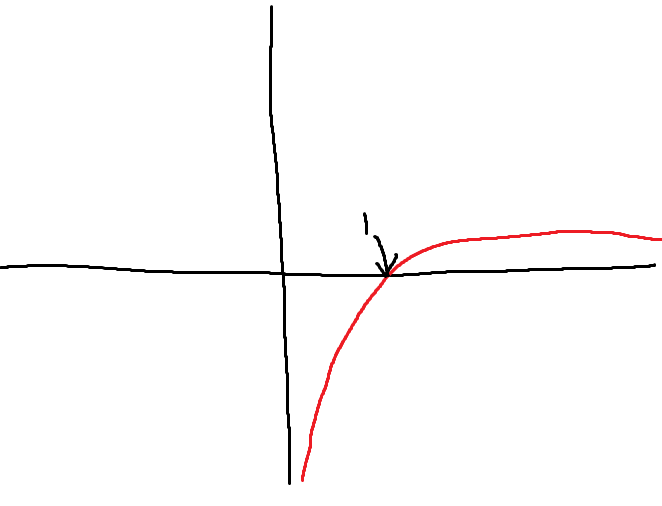
\includegraphics[width=\textwidth]{shittylogxoverx.png}

\begin{align*}
f(x) = & \ \frac{\log x}{x}\\
f'(x) = & \ - \frac{\log x - 1}{x^2} \\
f''(x) = & \ \frac{2 \log x -3}{x^3}
\end{align*}
$f$ is increasing on $(0, e)$ because $f'$ is positive on that interval. Similarly $f$ decreasing on $(e, \infty)$ because $f'$ is negative on that ray. $f$ has a local maxima/ global maxima at $e$ with $f(e) = \frac1e$. $f$ is concave down on $(0, e^\frac32)$ because $f''$ is negative on that interval. $f$ is concave up on $(e^\frac32,\infty)$ because $f''$ is positive on that ray. $f$ has a zero at 1 because $\log 1 = 0$. As $x$ goes to $\infty$, $f(x)$ also goes to $\infty$ because both $x \mapsto x$ and $x \mapsto \log x$ go to $\infty$. As $x$ goes to $\infty$, $f(x)$ goes to 0 because $\log x$ goes to $\infty$, while $\frac1x$ goes to 0. However it goes to 0 faster than $\log x$ goes to $\infty$, which can be verified using \textit{l'hopital's rule}.

b)

\begin{myproof}
\begin{align*}
\frac{\log(x^y)}{\log(y^x)} = \frac{y \log x}{x \log y} = \frac{\log x}{x} \frac{y}{\log y} = \frac{f(x)}{f(y)}
\end{align*}
ta-da!
\end{myproof}

c)

\begin{align*}
\pi^e < e^\pi
\end{align*}

\begin{myproof}
Consider for the sake of contradiction that $ e^\pi \leq \pi^e$. Because $\log$ is an increasing function $\log e^\pi \leq \log \pi^e$. This implies that 
\begin{align*}
1 \leq \frac{\log \pi^e}{\log e^\pi} = \frac{f(\pi)}{f(e)}
\end{align*}
However, if we take a look at the sketch of the graph, $f$ is decreasing on $(e, \infty)$. Thus $f(\pi) < f(e)$. However
\begin{align*}
1 \leq \frac{f(\pi)}{f(e)} \implies f(e) \leq f(\pi) \text{ \blitze}
\end{align*}
Aha, a contradiction. Bam, \textit{proof by picture}!
\end{myproof}

\newpage

3. a)

\begin{myproof}
We will prove this using strong induction on $n$. \nskip
Base Case: $n=1$. $\varphi(1) = \sum_{k=1}^1f(k) - \int_1^1f(x) \,dx = f(1)$ \nskip
$\varphi(2) = \sum_{k=1}^2f(k) - \int_1^2f(x)dx = f(1) + f(2) - \int_1^2f(x)\,dx$ \nskip
However, because $f$ is decreasing, we know that $f(1) > \int_1^2f(x) \,dx > f(2)$. Because the constant functions of $x \mapsto f(1) > f(x), \ \forall x \in (1,2)$, and $f(x) > x \mapsto f(2), \ \forall x \in (1,2)$. Thus, if we know
\begin{align*}
f(1) > \int_1^2f(x) \,dx > f(2)
\end{align*}
It easily follows that
\begin{align*}
f(2) < f(1) + f(2) - \int_1^2f(x)\,dx < f(1)
\end{align*}
And $f(1) = \varphi(1)$, making the base case true. \nskip
Induction Hypothesis: If $j < n$, then $\varphi (j+1) < \varphi (j)$. \nskip
Inductive Step: $\varphi(n) = f(n) + \varphi(n-1) - \int_{n-1}^nf(x) \,dx$ \nskip
$\varphi (n+1) = f(n+1) + \varphi (n) - \int_n^{n+1} f(x) \,dx$ \nskip
By the induction hypothesis $\varphi (n) < \varphi (n-1)$.
Because $f$ is decreasing, $f(n) > \int_n^{n+1}f(x) \,dx > f(n+1) $, and which implies that $f(n+1) - \int_n^{n+1}f(x) \,dx < 0$. Thus
\begin{align*}
\varphi(n) > f(n+1) + \varphi (n) - \int_n^{n+1}f(x) \,dx = \varphi (n+1)
\end{align*}
As desired.
\end{myproof}

b)

\begin{myproof}
We will prove this using strong induction on $n$. \nskip
Base Case: $n =2$
\begin{align*}
f(2) = \sum_{k=2}^2f(k) < \int_1^2f(x)dx < f(1) = \sum_{k=1}^1f(k)
\end{align*}
Therefore, the base is true. \nskip
Induction Hypothesis: If $j < n$, then 
\begin{align*}
\sum_{k=2}^jf(k) < \int_1^jf(x)dx < \sum_{k=1}^{j-1}f(k)
\end{align*}
Inductive Step: Because $x \mapsto f(n+1) < f$ on the interval $(n-1,n)$, then $\int_{n-1}^nf(x) \,dx > f(n+1)$. Thus by the induction hypothesis
\begin{align*}
\sum_{k=2}^{n-1} f(k) < \int_1^{n-1} f(x) \,dx
\end{align*}
Thus, it follows by above that 
\begin{align*}
\sum_{k=2}^n f(k) = f(n+1) + \sum_{k=2}^{n-1} f(k)  < \int_1^{n-1} f(x) \,dx + \int_{n-1}^n f(x) \,dx = \int_1^n f(x) \,dx
\end{align*}
Because $x \mapsto f(n-1) > f$ on the interval $(n-1,n)$, then $\int_{n-1}^n f(x) \,dx < f(n-1)$.
Thus, it follows by above that
\begin{align*}
\int_1^n f(x) \,dx = \int_1^{n-1} f(x) \,dx + \int_{n-1}^n f(x) \,dx < \sum_{k=1}^{n-2}f(k) + f(n-1) = \sum_{k=1}^{n-1} f(k)
\end{align*}
As desired.
\end{myproof}

c)

\begin{myproof}
We will prove this using strong induction on $n$. \nskip
Base Case: $n = 2$
\begin{align*}
f(2) < & \ \sum_{k=1}^2 f(k) - \int_1^2 f(x) \,dx \\
= & \ f(1) + f(2) - \int_1^2 f(x) \,dx \\
= & \varphi (2)
\end{align*}
We know this because $\int_1^2 f(x) \,dx < f(1)$. Similarly, we know that $\int_1^2 f(x) \,dx > f(2)$, implying
\begin{align*}
\varphi (2) = & \ f(1) + f(2) - \int_1^2 f(x) \,dx \\
 = & \ f(1)
\end{align*}
Therefore, the base case is true. \nskip
Induction Hypothesis: If $j<n$, then $f(j) < \varphi (j) < f(1)$ \nskip
Inductive Step: $\varphi (n) < f(1)$ is true because we have proven that $\varphi (n+1) < \varphi (n)$. Thus, we only have to prove that $f(n) < \varphi (n)$. Notice that because $f$ is decreasing $f(n) - \int_1^n f(x) \,dx >0$. Thus 
\begin{align*}
f(n) < \sum_{k=1}^{n-1} f(k) < \sum_{k=1}^{n-1} f(k) + f(n) - \int_1^n f(x) \,dx = \varphi (n)
\end{align*}
As desired.
\end{myproof}

\newpage

4. a)

\begin{myproof}
Notice that $f(x) = x^x \exp(-x^\lambda) = \exp(x \log (x) - x^\lambda)$. Notice that because the exponential is continuous
\begin{align*}
\lim_{x \to \infty} f(x) = \exp ( \lim_{x \to \infty} x \log x - x^\lambda )
\end{align*}
however
\begin{align*}
\lim_{x \to \infty} x \log x - x^\lambda = \lim_{x \to \infty} \frac{\frac{1}{x^\lambda}-\frac{1}{x \log x}}{\frac{1}{x^{\lambda+1} \log x}} \rightarrow \frac{0}{0}
\end{align*}
\begin{align*}
\frac{d}{dx}\Bigg( \frac{1}{x^\lambda}-\frac{1}{x \log x} \Bigg) = &  \ -\frac{\lambda }{x^{-\lambda -1}} - \frac{1}{x^2 \log  x} - \frac{1}{x^2 \log^2 x} \\
\frac{d}{dx} \Bigg( \frac{1}{x^{\lambda+1} \log x} \Bigg) = & \ - \frac{\lambda}{x^{-\lambda -2} \log x}+ \frac{1}{x^{-\lambda -2} \log^2 x} +  \frac{x^\lambda \log x}{x^{2\lambda+2} \log^2 x}
\end{align*}
\end{myproof}

b)

\begin{myproof}
We will show that $f(x) = \frac{x}{\sqrt{1-\cos x}}$ is not bounded, thus it is not integrable. \nskip
Consider
\begin{align*}
\lim_{x \to 2 \pi} \frac{x}{\sqrt{1-\cos x}} = & \ \lim_{x \to 2 \pi} x \frac{1}{\sqrt{\cos x - 1}} \\
= & \ \lim_{x \to 2 \pi} x \exp \Big( \log \Big( \frac{1}{\cos x - 1} \Big) \Big) \\
= & \ \lim_{x \to  2 \pi} x \exp \Big( -\frac12  \log \Big(\cos x - 1 \Big) \Big) \\
\end{align*}
But because the exponential function is continuous we can rewrite this as
\begin{align*}
\lim_{x \to 2 \pi} x \cdot \exp \Big(- \frac12 \lim_{x \to 2 \pi} \log \Big (\cos x -1 \Big) \Big)
\end{align*}
However, the logarithm is also continuous.
\begin{align*}
\lim_{x \to 2 \pi} x \cdot \exp \Big(- \frac12  \log \Big (\lim_{x \to 2 \pi} \cos x -1 \Big) \Big)
\end{align*}
However, as $x$ approaches $2 \pi$, $\cos x$ approaches $0$, which means that $ \log x$ goes to $-\infty$. Thus $\exp x$ goes to $\infty$ Which means the function is unbounded and thus, not integrable.
\end{myproof}

\newpage

5.

\begin{myproof}
We will prove using strong induction that $a_{2n-1} > a_{2n+1} > 0, \ \forall n \in \N$. \nskip Base Case: $n=0$ 
\begin{align*}
a_3 = & \ \int_0^{3\pi} f(x) \sin x \,dx \\
= & \ \int_0^{\pi} f(x) \sin x \,dx + \int_\pi^{2\pi} f(x) \sin x \,dx + \int_{2\pi}^{3\pi} f(x) \sin x \,dx
\end{align*}
but we know the last two terms are less than 0 but greater than $a_1$ because $f$ is decreasing and $\sin$ is negative on odd intervals of $\pi$. Thus
\begin{align*}
a_1 > \int_0^{\pi} f(x) \sin x \,dx + \int_\pi^{2\pi} f(x) \sin x \,dx + \int_{2\pi}^{3\pi} f(x) \sin x \,dx  = a_3 > 0
\end{align*}
Therefore, the base case is true. \nskip
Induction hypothesis: If $j < n$, then $a_{2j-1} > a_{2j+1}> 0$. \nskip
Inductive Step: 
\begin{align*}
a_{2n+1} = & \ \int_0^{(2n+1)\pi} \\
= & \ \int_0^{(2n-1)\pi} f(x) \sin x \,dx + \int_{(2n-1)\pi}^{(2n)\pi} f(x) \sin x \,dx + \int_{(2n)\pi}^{(2n+1)\pi} f(x) \sin x \,dx 
\end{align*}
However, the last two terms are less than 0 but greater than $a_{2n+1}$ because $f$ is decreasing, thus it easily follows that 
\begin{align*}
a_{(2n+1)} < a_{(2n-1)}
\end{align*}
We can similarly prove that $a_{2n-1} < a_{2n} < a_{2n+1}, \ \forall n \in \N$. Thus, consider $(a_n)_{n \in \N}$ and the subsequences $(a_{2n})_{n \in \N}$ and $(a_{2n-1})_{n \in \N}$. Because the odd subsequence is decreasing we know that
\begin{align*}
M := \lim_{x \to \infty} (a_{2n-1})
\end{align*}
exists by \textit{monotone convergence theorem}. The even sequence is also bounded above by $a_1$, thus  we know it also converges
\begin{align*}
m := \lim{x \to \infty} (a_{2n})
\end{align*}
because $\lim_{x \to \infty} f(x) = 0$, then the even and odd subsequences must converge somewhere in between $a_1$ and 0 because you can choose an $n$ such that their difference is arbitrarily small.
\end{myproof}

\end{flushleft}
\end{document}